\chapter{Background and Context}
\label{sec:background}

In this Chapter, we discuss the overall project of verifying behaviorally synthesized
designs, and how the certification of loop pipelining fits into
this project.  The reader interested in a thorough understanding of other
components of the project is welcome to review the prior
publications~\cite{rhcxy:atva-09,hxry:date-10}.

\section{Behavioral Synthesis}

Behavioral synthesis~\cite{lin:survey-97} is an automated compilation process where a behavioral synthesis tool ~\cite{spark,xpilot,legup}  takes an ESL description, together with a library of hardware resources. Analogous to a regular compiler,
the tool performs the standard lexical and syntax analysis to generate an intermediate representation (IR). The IR is then subjected to a number of
transformations which can be categorized into three phases as shown in Figure~\ref{fig:certification-framework}.

 \begin{enumerate}[--]
\item {\bf Compiler Transformations:} These include typical
  compiler operations, {\em e.g.,} dead-code elimination,
  constant propagation, loop unrolling, common subexpression elimination etc.  Furthermore, expensive operations ({\em e.g.,} division) may be replaced with simpler ones ({\em e.g.,} subtraction). A design may
  undergo hundreds of compiler transformations.
\item {\bf Scheduling Transformations:} Scheduling entails
  computing for each operation the clock cycle of its
  execution, accounting for hardware resource constraints
  and control/data dependencies.  Loop pipelining, the focus of our
  dissertation thesis, is a component of this phase.
\item {\bf Resource Allocation and Control Synthesis:} This phase
  involves mapping a hardware resource to each operation (%\eg, 
the
  ``{\tt +}'' operation may be mapped to a hardware adder), allocating
  registers to variables, and generating a controlling finite-state
  machine to implement the schedule.
\end{enumerate}
After the three phases above, the design can be expressed in
RTL.  The synthesized RTL may be subjected to further manual
tweaks to optimize for area, power, etc. Each of these transformations are non-trivial. The end result is a hardware implemtation which has a huge abstraction gap from the input ESL description. 

\section{Overall Certification Model for Behaviorally Synthesized Pipelines}

\begin{figure}[t!]
\begin{center}
\begin{tabular}{c}
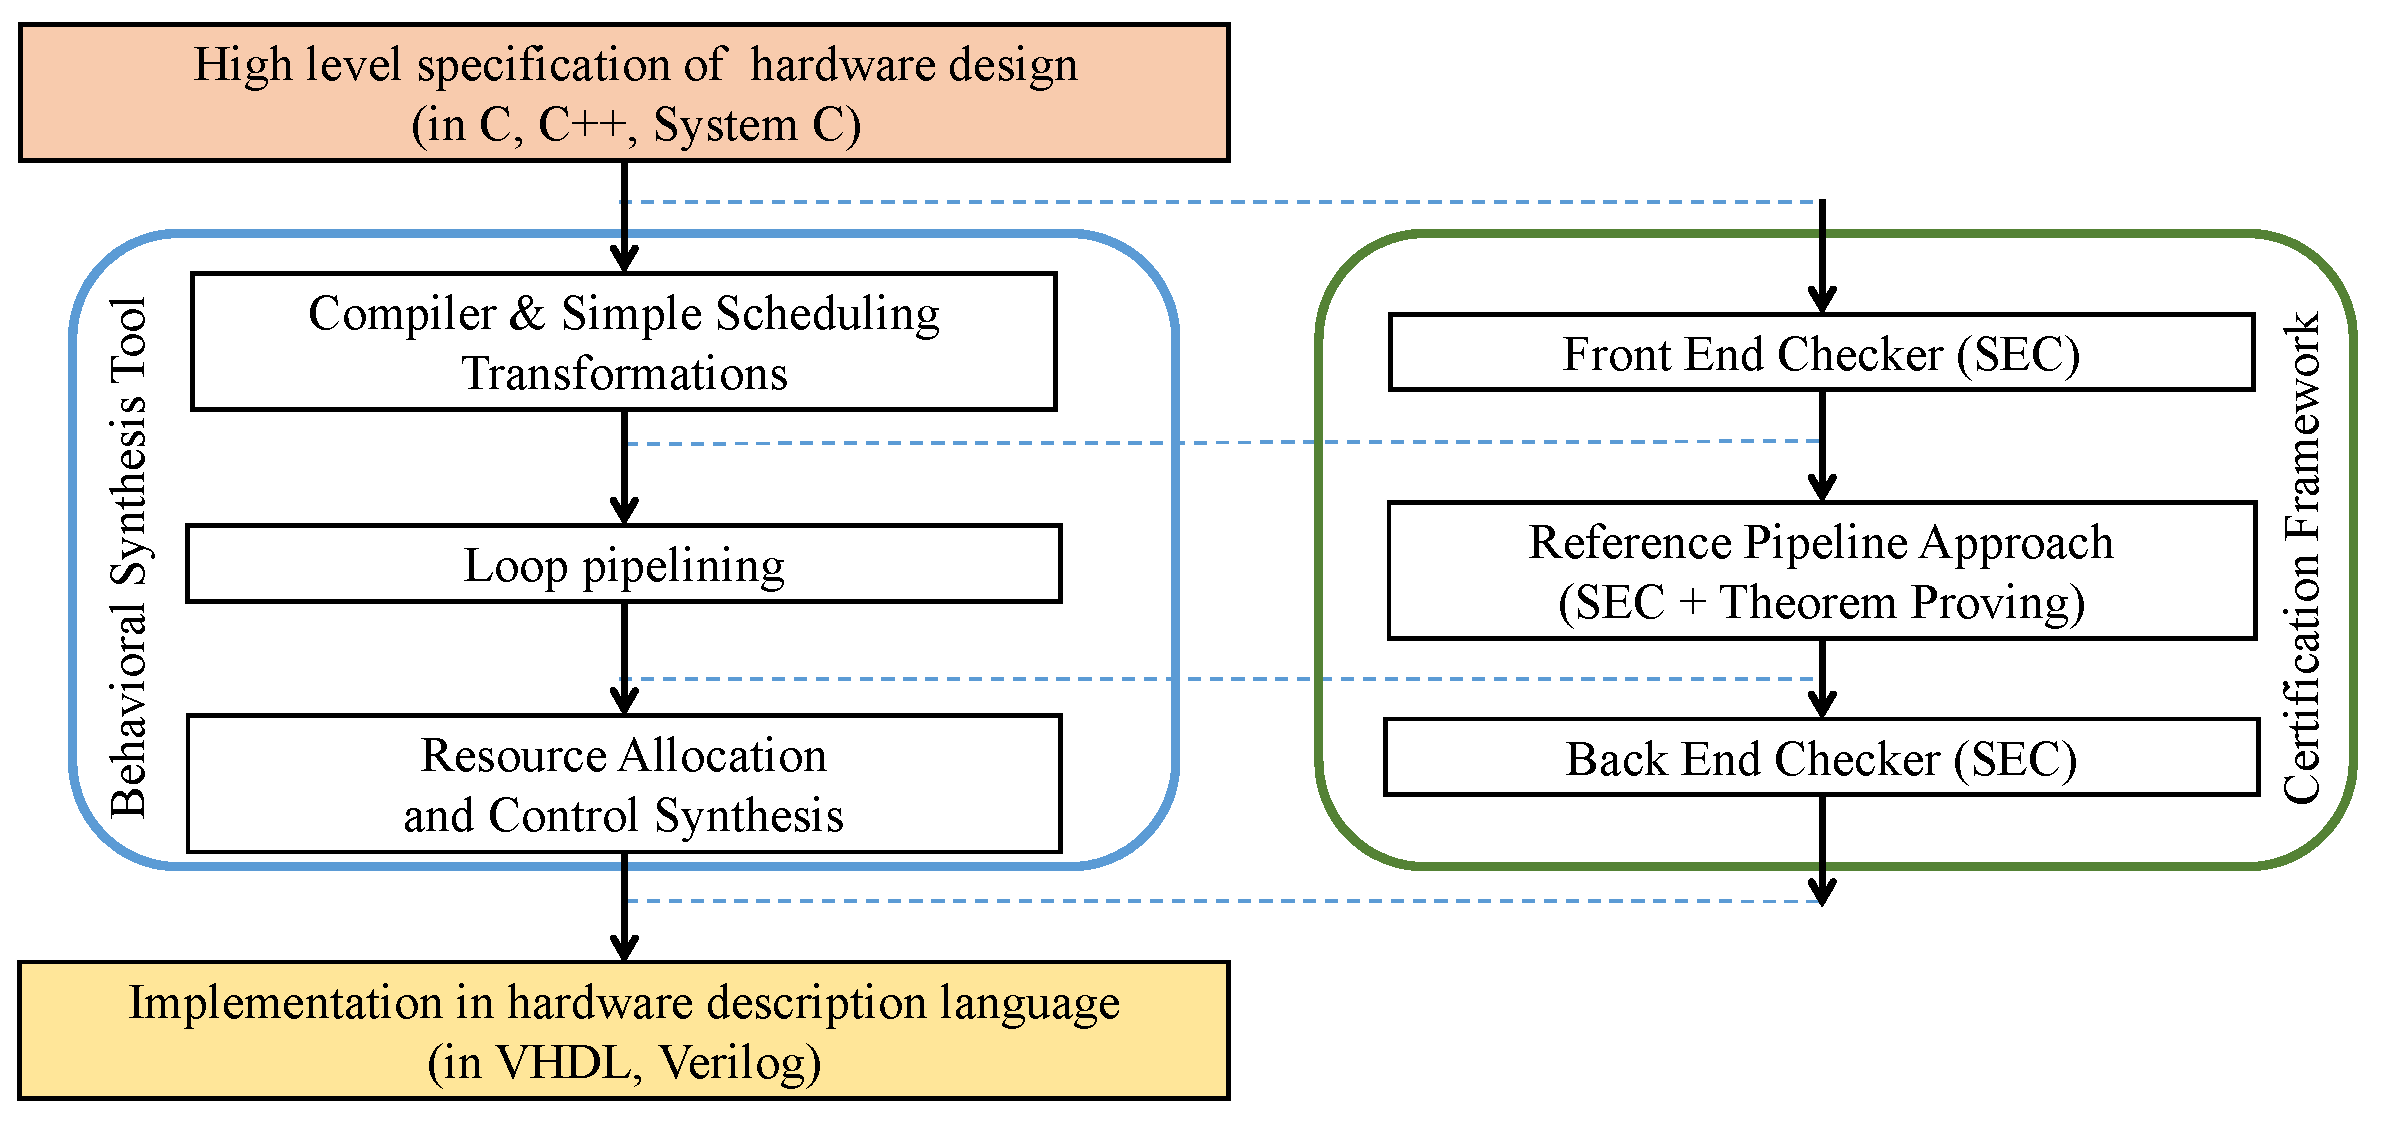
\includegraphics[height=2.8in]{fig-proposal/certification-framework}
\end{tabular}
\end{center}
\caption{Certification Model for Behaviorally Synthesized Pipelines}
\label{fig:certification-framework}
\end{figure}

The overall goal of the project is to provide a mechanized framework
for certifying hardware designs synthesized from ESL specifications by
commercial behavioral synthesis tools.
One obvious approach is to apply standard verification techniques (%\eg, 
SEC or
theorem proving) on the synthesized RTL itself.
Unfortunately, such a methodology is not practical.
As mentioned earlier, the large gap in abstraction
between the ESL and RTL descriptions means that there is little
correspondence in internal variables between the two.  Consequently,
direct SEC between the two reduces to cost-prohibitive computation of
input-output equivalence. On the other side, applying theorem proving
is also troublesome since extensive manual effort is necessary and
this effort needs to be replicated for each different synthesized
design. It is also infeasible to
directly certify the implementation of the {\em synthesis tool} via
theorem proving.  In addition to being highly complex and thus
potentially requiring prohibitive effort to formally verify with any
theorem prover, the implementations are typically closed-source and
closely guarded by EDA vendors and thus out of reach of external
automated reasoning communities.

To address this problem, previous work developed two key SEC
solutions, which we will refer to below as {\em Back-end} and {\em
Front-end}.  We then discuss the gap between them, which is being
filled by theorem proving efforts in this dissertation. The certfication model 
is illustrated in Figure~\ref{fig:certification-framework}.
\medskip

\noindent {\bf Back-end SEC:} The key insight behind
back-end SEC is that automated SEC techniques, while
ineffective for directly comparing synthesized RTL with the
top-level ESL description, are actually suitable to compare
the RTL with the intermediate representation (IR) generated
by the tools after the high-level (compiler and scheduling)
transformations have been applied.  In particular,
operation-to-resource mappings generated by the synthesis
tool provide the requisite correspondence between internal
variables of the IR and RTL.  Furthermore, a key insight is
that while the implementations of transformations are
unavailable for commercial EDA tools, most tools provide
these IRs after each transformation application together
with some other auxiliary information.  To exploit these, an
SEC algorithm was developed between the IR (extracted from
synthesis tool flow after these transformations) and
RTL~\cite{rhcxy:atva-09,hxry:date-10,kechengthesis,Yang2013}. 
The approach scales
to tens of thousands of lines of synthesized RTL.

\medskip

\noindent {\bf Front-end SEC:} Of course the back-end SEC
above is only meaningful if we can certify that the input
ESL indeed corresponds to the extracted IR produced after
the compiler and scheduling transformations applied in the
first two phases of synthesis. To address this, another SEC
technique was developed to compare two IRs~\cite{zhenkun:iccd-13,zhenkun2,zhenkun3}.  The idea then
is to obtain the sequence of intermediate representations
$\mbox{IR}_0,\ldots,\mbox{IR}_n$ generated by the compiler
and scheduling transformations, and compare each pair of
consecutive IRs with this new algorithm.  Then back-end SEC
can be used to compare $\mbox{IR}_n$ with the synthesized
RTL, completing the flow.

\bigskip

\noindent {\bf A Methodology Gap:} Unfortunately, the front-end SEC
algorithm can only compare two IRs that are structurally close.  If a
transformation significantly transforms the structure of an IR then
the heuristics for detecting corresponding variables between the two
IRs will not succeed, causing equivalence checking to fail.
Unfortunately, loop pipelining falls in the category of
transformations that significantly changes the structure of the IR.
It is a quintessential transformation that changes the control/data
flow and introduces additional control structures (%\eg, 
to eliminate
hazards).  This makes front-end SEC infeasible for its certification.
%On the other hand, it is also a complex and error-prone
%transformation, and ubiquitous across different behavioral synthesis
%tools. 
Furthermore, most commercial implementations are of course
proprietary and consequently not available to us for review; applying
theorem proving on those implementations is not viable from a
methodology perspective.  Thus a specialized approach is warranted for
handling its certification.

\section{A Reference Pipeline Approach}
\label{subsec:reference-pipeline}

\begin{figure}[t!]
\begin{center}
\begin{tabular}{c}
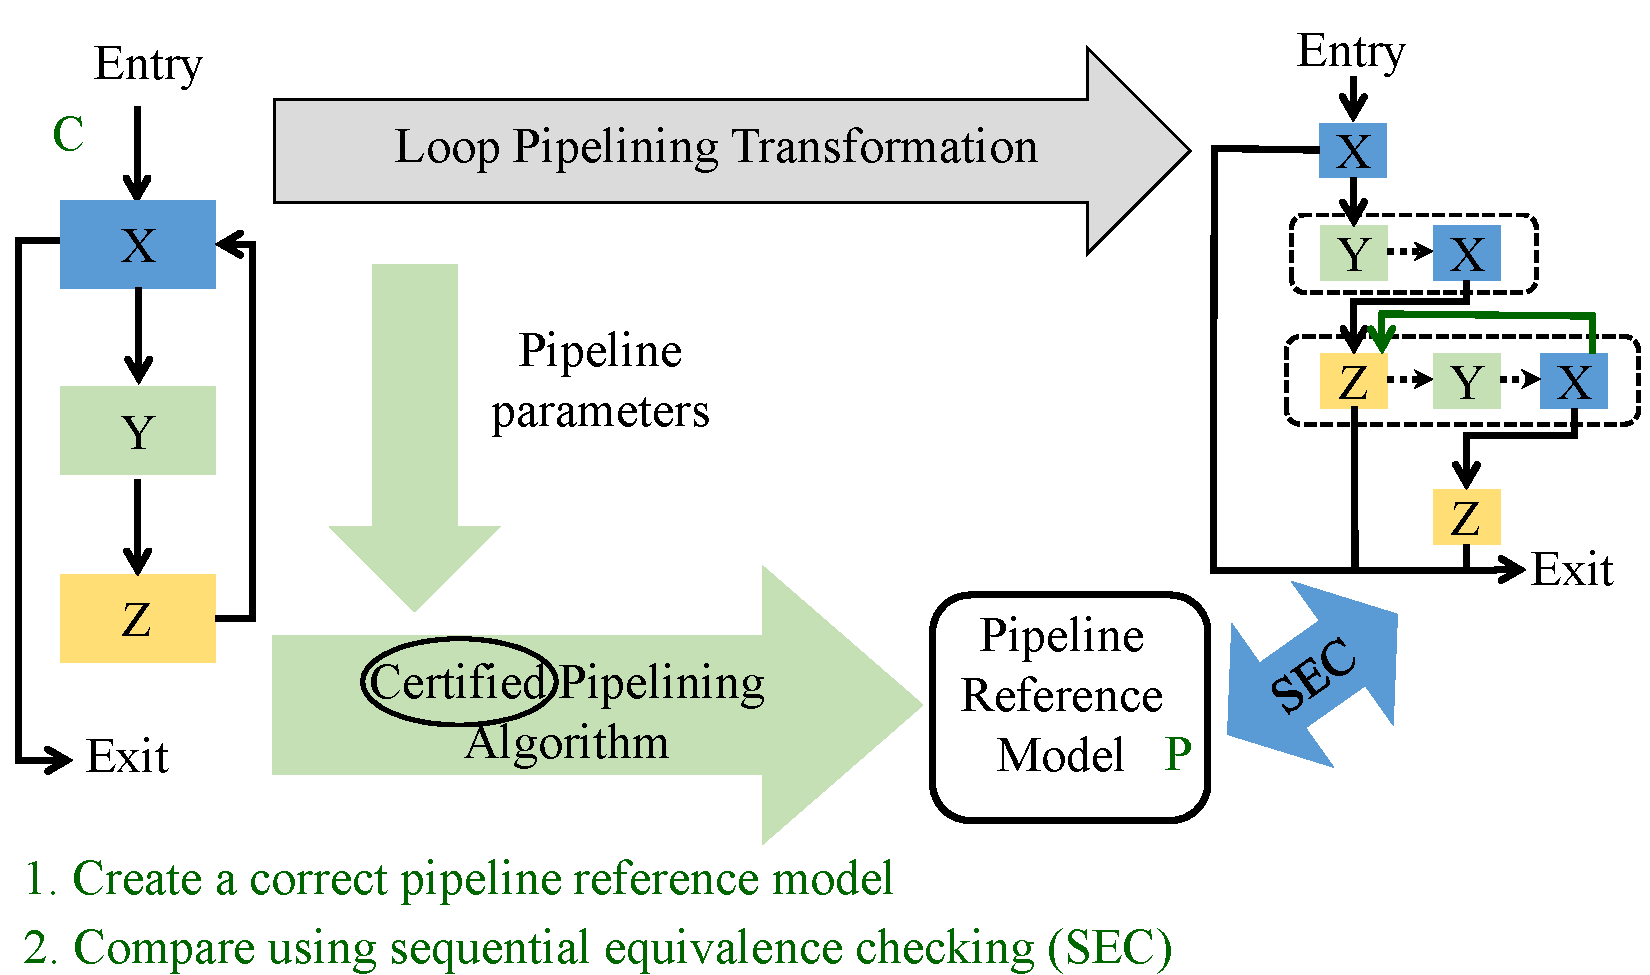
\includegraphics[height=3in]{fig-proposal/ref-pipeline-approach}
\end{tabular}
\end{center}
\caption{Certifying Loop Pipelining Algorithm using SEC and Theorem Proving}
\label{fig:ref-pipeline-approach}
\end{figure}

To develop a specialized approach for pipelines, a key observation
is that while the transformation {\em implementation} is inaccessible
to us, commercial synthesis tools typically generates a report
specifying pipeline parameters (%\eg, 
pipeline interval, number of loop
iterations pipelined, etc.).  The approach (c.f. Figure~\ref{fig:ref-pipeline-approach})
then is to develop an
algorithm that takes as inputs these parameters and an IR ${\cal{C}}$
for the design before pipelining, and generates a {\em reference
  pipelined IR} ${\cal{P}}$.  Note that this algorithm would be much simpler
than that employed during synthesis; while the former includes
advanced heuristics to {\em compute} pipeline parameters (like
pipeline interval, number of iterations pipelined etc.), this algorithm would merely use
the values provided by its report.  To certify a synthesized RTL with
pipelines, it is sufficient to (1)~check that the {\em given algorithm} can
generate a pipeline ${\cal{P}}$ for the parameters reported by
synthesis, (2)~use SEC to compare ${\cal{P}}$ with the synthesized
RTL, and (3)~prove (using theorem proving) the correctness of this
algorithm.

A previous work~\cite{hrx:dac-12} justified the viability of
steps 1 and 2 above; such a reference pipeline generation algorithm
was developed and used to successfully compare a variety of pipelined
designs across various application domains.  This suggested that the
approach of using a reference implementation is viable for certifying
industrial strength behaviorally synthesized pipelines.  However, a key (and perhaps the
most complicated) component of the approach was missing.  The
algorithm was not verified (indeed, not implemented in a formal
language), rendering the ``certification'' flow unsound.

The unsoundness mentioned above is not just an academic notion.  
The approach showed no systematic approach for
creating the reference pipeline generation algorithm.  In
fact, the specific reference algorithm developed was in fact
heavily influenced by the synthesis tool under consideration
(AutoESL), and highly complex. In
fact, merely by going through the formalization process and thinking
about necessary invariants, we have already found a bug in
the implementation of the algorithm.  
Thus it is critical to develop a mechanized proof of
correctness for this implementation.  Unfortunately, it is not easy to
verify the original pipeline generation algorithm as written.  Its
author was an expert in behavioral synthesis but not in program
verification or theorem proving; consequently, the algorithm, while
simpler than the one implemented in a synthesis tool, was still a highly
complex piece of code.  In particular, since it was not written with
correctness certification in mind, it is difficult to decompose the algorithm into
manageable pieces with nice invariants.

One way to address this problem is to ``buckle down'' and
verify the pipeline generation algorithm (and fixing the
bugs found in the process).  However, a key insight in our
case is that we can get away without verifying such a
complex implementation.  After all, there is nothing
``sacred'' about this specific algorithm for pipeline
generation: given the steps described above, {\em any}
verifiable pipeline generation algorithm would
suffice.\footnote{Note that our algorithm {\em must} create
  a pipeline in accordance with the pipeline parameters
  obtained from the behavioral synthesis tools; otherwise we may
  fail to certify correct designs. However, in practice, we
  have not found this to be a problem.}  Thus the approach
of our dissertation can be viewed as a rational deconstruction of
the pipeline synthesis algorithm of the previous work.  We
identify the key invariant that we need to maintain for
proving computational equivalence between the pipelined and
un-pipelined loops and design an algorithm to explicitly
maintain that invariant.

We discuss the previously proposed algorithm in Chapter~\ref{sec:challenges}
such that we can draw a comparison and better understand the differences
in our implementation of loop pipelining algorithm due to our need to formally certify it.


%We start with a brief summary of behavioral synthesis, highlighting
%the aspects necessary to understand our dissertation thesis.
%the rest of our presentation.
%Note that behavioral synthesis is a complex technology whose
%description is far beyond the scope of this paper.  However, there are
%several behavioral synthesis tools available, including both
%commercial and academic ones, with extensive manuals, documentations
%and tutorials providing user-level description of their
%workings~\cite{spark,xpilot,legup}, and we encourage the
%interested reader to review these materials for further information.

%At a high level, a behavioral synthesis tool can be best viewed as a
%``compiler'' that takes an ESL description and generates RTL.
